\documentclass[technote,a4paper]{IEEEtran}
\usepackage{amssymb, amsmath} % needed for math

\usepackage[a-1b]{pdfx}
\usepackage{filecontents}
\begin{filecontents*}{\jobname.xmpdata}
    \Keywords{recognition\sep machine learning\sep neural networks\sep symbols\sep multilayer perceptron}
    \Title{Pixel-wise Segmentation of Street with Neural Networks}
    \Author{Martin Thoma, Marvin Teichmann, Sebastian Bittel, Vitali Kaiser}
    \Org{Forschungszentrum Informatik (FZI)}
    \Doi{}
\end{filecontents*}

\RequirePackage{ifpdf}
\ifpdf \PassOptionsToPackage{pdfpagelabels}{hyperref} \fi
\RequirePackage{hyperref}
\usepackage{parskip}
\usepackage[pdftex,final]{graphicx}
\usepackage{csquotes}
\usepackage{braket}
\usepackage{booktabs}
\usepackage{multirow}
\usepackage{pgfplots}
\usepackage{wasysym}
\usepackage{float}
\usepackage{caption}
\usepackage{subcaption}
% \captionsetup{belowskip=12pt,aboveskip=4pt}
\makeatletter
\newcommand\mynobreakpar{\par\nobreak\@afterheading}
\makeatother
\usepackage[noadjust]{cite}
\usepackage[nameinlink,noabbrev]{cleveref} % has to be after hyperref, nthe l.137 ...eam attr{/N 4}  file{sRGBIEC1966-2.1.icmorem, amsthm
\usepackage[binary-units,group-separator={,}]{siunitx}
\sisetup{per-mode=fraction,binary-units=true}
\DeclareSIUnit\pixel{px}
\usepackage{glossaries}
\loadglsentries[main]{glossary}
\makeglossaries

\title{Pixel-wise Segmentation of Street with Neural Networks}
\author{Sebastian Bittel, Vitali Kaiser, Marvin Teichmann, Martin Thoma}

\hypersetup{
	pdfauthor   = {Sebastian Bittel\sep Vitali Kaiser\sep Marvin Teichmann\sep Martin Thoma},
	pdfkeywords = {recognition\sep machine learning\sep neural networks\sep classification\sep multilayer perceptron\sep deep learning},
	pdfsubject  = {Recognition},
	pdftitle    = {Pixel-wise Segmentation of Street with Neural Networks},
}


\crefname{table}{Table}{Tables}
\crefname{figure}{Figure}{Figures}

%%%%%%%%%%%%%%%%%%%%%%%%%%%%%%%%%%%%%%%%%%%%%%%%%%%%%%%%%%%%%%%%%%%%%
% Begin document                                                    %
%%%%%%%%%%%%%%%%%%%%%%%%%%%%%%%%%%%%%%%%%%%%%%%%%%%%%%%%%%%%%%%%%%%%%
\begin{document}
\maketitle
\begin{abstract}
Pixel-wise street segmentation of photographs taken from a drivers perspective
is important for self-driving cars and can also support other object
recognition tasks. A framework called SST was developed to examine the accuracy
and execution time of different neural networks. The best neural network
achieved an $F_1$-score of \SI{89.5}{\percent} with a simple feedforward
neural network which trained to solve a regression task.
\end{abstract}

%!TEX root = pixel-wise-street-segmentation.tex

\section{Introduction}
Pixel-wise segmentation of street is an important part of assisted and
autonomous driving~\cite{Tarel2009}. It can help to understand road scenes and
reduce the space to search for lane markings. Traditionally, road segmentation
is done with computer vision methods such as watershed
transformation~\cite{Beucher1990}. Recent advances in deep neural networks,
escpecially in computer vision, suggest that \glspl{CNN} might perform better
on road segmentation tasks then those traditional approaches.
%!TEX root = pixel-wise-street-segmentation.tex

\section{Related Work}\label{sec:related-work}
Road segmentation is a subproblem of general scene parsing or segmentation. In scene parsing every object in a scene is classified pixelwise with a label. Whereas in road segmentation often only two classes exist and more assumptions can be applied.\\
In the first publication roads were usually annotated by color-based histogram approaches and specific model knowledge. Examples are the in 1994 introduced approach \cite{Beucher1990} using the watershed algorithm or \cite{aly2008real} where roads were annoted indirectly by lane markings found with a hough transformation.\\
Later insights of general scene parsing where transferred and more generic approaches like \cite{6182716} have achieved remarkable results with a Markov Random Field (MRF) and superpixels.\\
The impressive classification results of CNNs like AlexNet \cite{krizhevsky2012imagenet} or GoogleLeNet \cite{SzegedyLJSRAEVR14} during the the Google ImageNet LSVRC-2010 contest, made CNNs interesting for all kinds of computer vision problems like e.g. segmentation. \\
With \cite{long2014fully} Long and his team introduced a method for general scene parsing based on Fully Convolutional Networks (FCNs) and deconvolutional layer.\\
This approach is used as a blueprint to our implementation, described in \cref{sec:model}. Therefore the main concepts are introduced at the end of this section.\\
Instead of creating a new model, they converted existing classifaction CNNs like AlexNet or GoogleLeNet into FCNs. The obtained heatmaps for every class where calculated for multiple resolutions and upscaled with deconvolution layer interpolation to the original resolution.
With a fully connected convolutional layer in the end, the multiple outputs are combined into one classification heatmap for every class.\\

In \cite{mohan2014deep} a approach is presented, which makes also use of a CNNs in combination with deconvolution. In comparison to Long's network, among others it is less deep and uses less convolutional then deconvolutional layers. Furthermore the input image is divided in multiple patches and for each patch a separate neural network was trained. Their model achieved the best-recorded result on the same data set we use, which is described in \cref{sec:datasets}.    

\subsection{CNN}
A CNN is a feed forward neural network with at least one convolutional layer. The neurons of convolutional layer... 

\subsection{FCN}
Is CNN where bla.
\begin{figure}[htb]
	\centering
	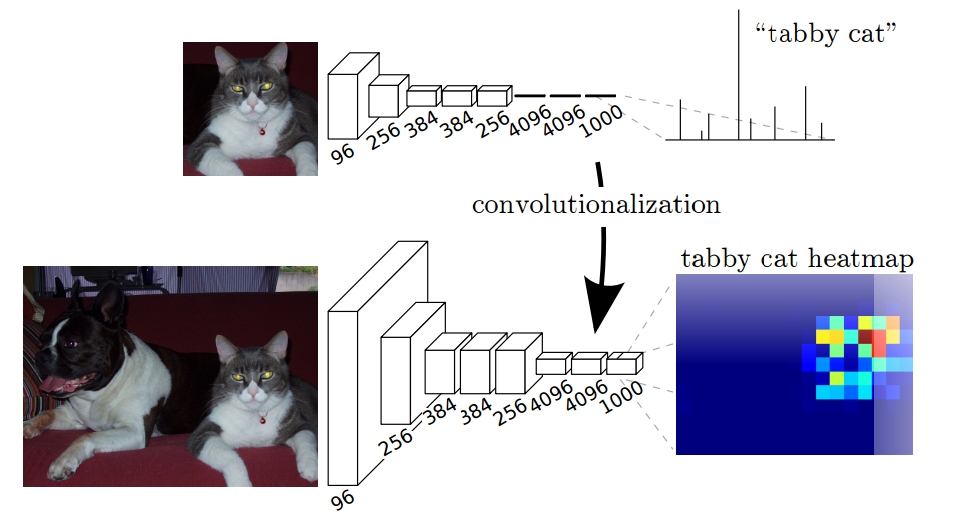
\includegraphics[width=9cm]{figures/fcnn}
	\caption{Comparison if a CNN for classifaction (top) and a FCN which creates a heatmap (bottom). \cite{long2014fully}}
\end{figure}

\subsection{Fully connected convolutional layer}
A fully connected convolutional layer is a regular convolutional layer in size of the input. Consequentially the weight matrix covers every input neuron. Long noted in \cite{long2014fully} that it is the two dimensional equivalent to fully connected layer in a classification CNN.

\subsection{Deconvolutional Layer}
Deconvolutions are inverse convolutions. In context of neural networks the function for forward and backward calculation are just switched. That results in a layer....

%!TEX root = pixel-wise-street-segmentation.tex

\section{Frameworks}\label{sec:frameworks}
nolearn was used in combination with Lasagne~\cite{sander_dieleman_2015_27878}
to train the models. Lasagne is based on Theano~\cite{Bergstra2010}. We also
used Caffe~\cite{Jia2014} for \glspl{CNN}, but skipped that approach as the
framework crashed very often for different training approaches without giving
meaningful error messages.

Theano is a Python library which allows symbolic computation of derivatives as
well as automatic generation of GPU code. This is used to calculate the weight
update function for arbitrary feed-forward networks. Lasagne makes using Theano
simpler by providing some basic layer types with their update function and
nolearn adds some syntactic sugar.
%!TEX root = pixel-wise-street-segmentation.tex

\section{SST}\label{sec:sst}
\Gls{sst} is a Python package hosted on \gls{PyPI} and developed on GitHub. It
makes use of Lasagne (see \cref{sec:frameworks}).

\subsection{Installation}
\verb+sst+ can be installed via \verb+pip install sst+. To make the
installation as simple as possible, this does not install all requirements.
\verb+sst selfcheck+ gives the user the possibility to check which packages
are still required and manually install them.

\subsection{Functionality}
\verb+sst+ makes use of Python files for neural network definitions. Those
models have to have a \verb+generate_nnet(feature_vectors)+ function which
returns an object with a \verb+fit(features, labels)+ method, a
\verb+predict(feature_vector)+ method and a
\verb+predict_proba(feature_vector)+ method. This is typically achieved by
returning a \verb+nolearn+ model object. The Python network definition file
has to have two global variables: \verb+patch_size+ (a positive integer) and
\verb+fully+ (a Boolean). The first variable is the patch size expected by the
neural network, the second variable indicates if the neural network was trained
to classify each pixel of the complete patch (\verb+fully = True+) or only the
center pixel (\verb+fully = False+).

\verb+sst --help+ shows all subcommands. The subcommands are

\begin{itemize}
    \item \verb+selfcheck+: Test which components or Python packages are
                            missing and have to be installed to be able to use
                            all features of \verb+sst+.
    \item \verb+train+: Train a neural network.
    \item \verb+eval+: Evaluate a trained network on a photograph and also
                       generate an overlay image of the segmentation and the
                       data photograph.
    \item \verb+serve+: Start a web server which lets the user choose images
                        from the local file system to predict the label and to
                        show overlays.
    \item \verb+view+: Show all information about an existing model.
    \item \verb+video+: Generate a video.
\end{itemize}
%!TEX root = pixel-wise-street-segmentation.tex

\subsection{Data Sets}\label{sec:datasets}
The KITTI Road Estimation data set~\cite{Fritsch2013} was used for training of
the models and for obtaining the experimental results reported in
\cref{sec:evaluation}.

The left color image base kit contains a training and a test set. All photos
are in an urban environment. The training set has 95~photos with land markings
(um), 96~photos with multiple lane markings (umm) and 98~photos where the
street has no lane markings (uu). The test set has 96~um~photos, 94~umm~photos
and 100~uu~photos.

The width of all photos is in $\Set{1226, 1238, 1241, 1242}$, the height is in
$\Set{370, 374, 375, 376}$.

The data photos are given as 8-bit color RGB PNG files. The labels (ground
truth) are given as images of the same size as the data image, but with only
three colors: red (\verb+#ff0000+), magenta (\verb+#ff00ff+) for street and
black (\verb+#000000+) for other streets than the one the car is on.
%!TEX root = pixel-wise-street-segmentation.tex

\section{Used models}\label{sec:model}

We have implemented two approaches to tackle  the street segmentation problem.
We have used a sliding window approach which is based on a classification
network and a regression approach. Both models are detailed in the following
section.

\subsection{The Sliding Window Approach}
Traditionally neural networks are used for classification tasks. As
described in \cref{sec:related-work} they deliver impressive results. Our first
approach is a sliding window model, which exploits the classification strength
of deep neural networks.

\subsubsection{Definition of the Classification Problem}
We trained a neural network to solve the following binary classification
problem:

\fbox{
    \begin{tabular}{l l}
        \multicolumn{2}{l}{\textbf{Classification Problem}} \\
        \textit{Input:} & A $n \times n$ 3-channel pixel image section.\\
        \textit{Output:} & Decide whether the center pixel is street.
    \end{tabular}
}

For $n$ we used $51$. This constant was chosen as we ran into GPU memory
problems when training on higher values of $n$. Our classification approach is
visualized in \cref{fig:figure}.

\begin{figure}[H]
    \centering
    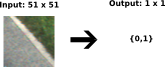
\includegraphics[width=0.5\columnwidth]{figures/models/sliding_window.png}
    \caption{Visualization of the classification problem solved by our neural network.}%
\label{fig:figure}
\end{figure}


\subsubsection{Net Topology}
The problem defined above can be tackled with any of the well known
classification networks such as GoogLeNet or AlexNet. For our solution we
designed our own network detailed in \cref{tab:topo}. The small size of only
three hidden layers was chosen as our experiments showed that small networks
perform better than networks with more layers. One reason for this is that the
amount of labeled images is rather small. Hence smaller nets generalize much
better. Secondly, the binary decision task of recognizing street is much
simpler than detailed image classification. This simplicity does also reflect
in the net topology.

\begin{table}[H]
    \normalsize
    \centering
\begin{tabular}{r  l l}
    \toprule
    \textbf{Layer} & \textbf{Type}  & \textbf{Shape}  \\
    \midrule
    0     & Input &  $51 \times 51 \times 3$ \\
    1     & Convolution & 10 filter  each $5 \times 5$ \\
    2     & Convolution & 10 filter  each $5 \times 5$  \\
    3     & Pooling     & $2 \times 2$ \\
    4     & Output     & $1$ \\
    \bottomrule
\end{tabular}
\caption{Topology of the classification network.}
\label{tab:topo}
\end{table}


\subsubsection{Training}
The training data for this classification problem can be easily obtained by
modifying the original training data. One advantage of our approach is that we
get a lot of training data out of each image. In theory, we get one (distinct)
datum for each pixel in each training image. However, it is not useful to
actually use all of this data as patches which are close to each other and thus
are very similar. Hence the information gain of including these patches is very
small. On the other hand, if we generate an image section for each pixel we
obtain more data than the memory of our GPU can handle. We therefore introduced
a training stride. A stride of $s$ results in the center pixels having a
distance of $s$ in height and with to the next sections center pixel. This is
important in the section generation step before training as well as for the
pixel-wise classification. The overlap of two adjacent images is hence reduced
to $n-s$, where $n \times n$ is the size of each image section. Empirical
evaluations indicated that $s=10$ is a good default value for the trainings
stride.

\subsubsection{Evaluation}
In order to apply a classification network on the segmentation problem we used
the well known sliding window approach. The main idea is to apply the
classification network on each pixel $p$ of the input image by generating the
$n \times n$ image section with center pixel $p$. We use padding to be able to
apply the method to pixels close to the border. \Cref{fig:stride2} shows the
result of this approach.

\begin{figure}[H]
    \centering
    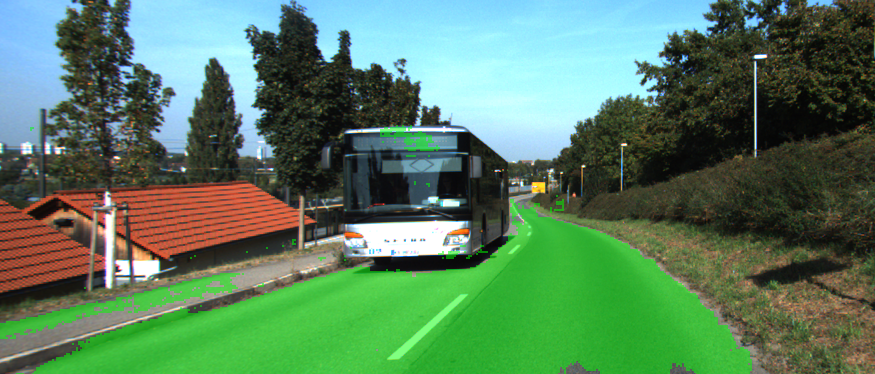
\includegraphics[width=\columnwidth]{figures/models/testing2-um_32_sliding_stride2.png}
    \caption{Using the sliding window approach with a stride of $s=2$.}%
\label{fig:stride2}
\end{figure}

The main disadvantage of this approach is the impractical runtime. For a
1~megapixel image we need to run 1~million classifications. This leads to a
runtime of almost two~minutes with our hardware. In order to reduce the
evaluation time we introduced an evaluation stride $s$. Similar to the training
stride we skip $s-1$ pixels in each dimension. This increases the evaluation
speed by a factor of $s^2$. For the sliding window approach we found that a
stride of $s = 10$ is a reasonable trade-off between speed and quality.
\Cref{fig:stride10} shows the result of the sliding window approach with a
stride of $s=10$.



\begin{figure}[H]
    \centering
    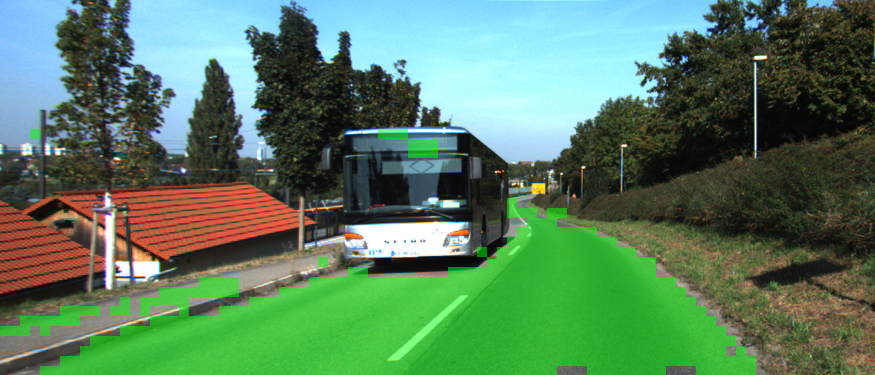
\includegraphics[width=\columnwidth]{figures/models/testing2-um_32_sliding_stride10.png}
    \caption{Using the sliding window approach with a stride of $s=10$.}%
\label{fig:stride10}
\end{figure}


\subsection{The Regression Approach}
The main disadvantage of our sliding window approach is that the segmentation
becomes very coarse with higher values for the stride $s$. To overcome this
problem we designed a regression neural networks which is able to classify each
pixel independently.

\subsubsection{Definition of the Regression Problem}
We trained a neural network to solve the following regression problem:

\fbox{
    \begin{tabular}{l l}
        \multicolumn{2}{l}{\textbf{Regression Problem}} \\
        \textit{Input:} & A $n \times n$ 3-channel pixel image section.\\
        \textit{Output:} & A $n \times n$ label.
    \end{tabular}
}

where the net is trained to minimize the mean squared error of the output. The
output of the regression net is continuous. We round the output to obtain a
binary classification. \Cref{fig:reg} visualizes our regression approach.

\begin{figure}[H]
    \centering
    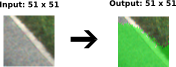
\includegraphics[width=0.5\columnwidth]{figures/models/fully-conv.png}
    \caption{Visualization of the regression approach.}%
\label{fig:reg}
\end{figure}

The goal is to choose $n$ as big as possible as $n^2$ is the number of pixels
which can be classified at once. However, due to GPU memory limitations we
cannot train a network with $n > 51$.


\subsubsection{Net Topology}
Similar to the classification approach our experiments show that a simple net
topologies work best. The topology we used is detailed in \cref{tab:topo2}.

\begin{table}[H]
    \normalsize
    \centering
    \begin{tabular}{r l l}
        \toprule
        \textbf{Layer} & \textbf{Type}  & \textbf{Shape}  \\
        \midrule
        0     & Input &  $51 \times 51 \times 3$ \\
        1     & Convolution & 10 filter  each $5 \times 5$ \\
        2     & Convolution & 1 filter $51 \times 51$  \\
        3     & Reshape (Flatten) & $51 \times 51$ \\
        4     & Output     & $2601\footnotemark \times 1$\\
        \bottomrule
    \end{tabular}
    \caption{Topology of the regression network.}%
\label{tab:topo2}
\end{table}
\footnotetext{The shape of $2601 \times 1$ is a result of flattening the $51 \times 51$ image patch. This is only necessary due to tooling support.}


\subsubsection{Training}
Training of the regression model can be implemented analogously to the
classification model. We use overlapping image section again to get as much
information out of the data as possible.

\subsubsection{Evaluation}
In order to evaluate a whole image using the regression approach we divide the
image into patches of size $n \times n$ and evaluate each patch individually.
The output is shown in \cref{fig:reg_stride2}. The result is quite impressive,
especially regarding the overall runtime of about $\SI{0.18}{\second}$ as shown
in \cref{tab:runtime}.

\begin{figure}[tbp]
    \centering
    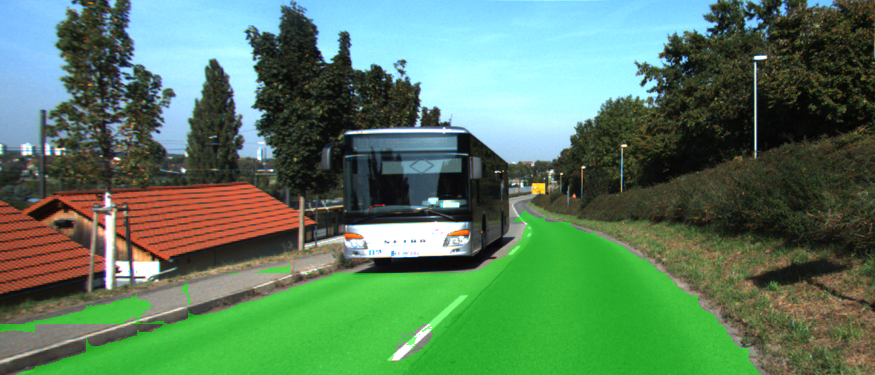
\includegraphics[width=\columnwidth]{figures/models/testing2-um_32_conv_stride51.png}
    \caption{Using regression approach with stride $s=51$}%
\label{fig:reg_stride2}
\end{figure}


One observation is, that the segmentation works better in the center of each
patch. The neural network does not have good information close to the border of
each image section. To overcome this problem we use an evaluation stride again.
This introduces an overlap between each image patch. A pixel $p$ is then
segmented according to the patch whose center is closer to $p$.


\begin{figure}[tbp]
    \centering
    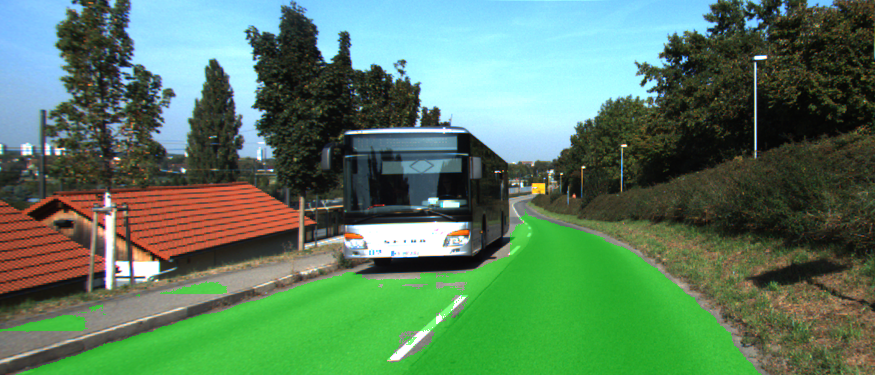
\includegraphics[width=\columnwidth]{figures/models/testing2-um_32_conv_stride37.png}
    \caption{Using regression approach with stride $s=37$}%
\label{fig:reg_stride37}
\end{figure}

\Cref{fig:reg_stride37} shows the output when using a stride of 37. We see that
the edge of the street is classified slightly better. In order to archive this
effect a rather big stride between 37~and~47 is already sufficient. In the
regression approach there is no measurable benefit of using strides below 37.

%!TEX root = pixel-wise-street-segmentation.tex

\section{Experimental Results}\label{sec:evaluation}

In this section we discuss the experimental results of the models
presented in \cref{sec:model}. First, we evaluate the two different
models. Second, we compare our best one to the work of
Mohan~\cite{Tarel2009} (which is ranked on place~1 at KITTI road
segmentation~\cite{Tarel2009}). The KITTI Road Estimation data set is the basis
of our experiments (see \cref{sec:datasets}). \\
To be able to evaluate different approaches we used only the
training data of the KITTI data set, as the ground truth for the test data is
not publicly available. We splitted the training data beforehand 20 to 80
(test/training) in order to be able to measure our performance. Our best model
was submitted for the official KITTI evaluation
(\href{http://www.cvlibs.net/datasets/kitti/eval_road.php}{www.cvlibs.net/datasets/kitti/eval\_road.php})


Our goal was to achieve an adequate classification performance while staying
within a time frame of \textbf{\SI{20}{\milli\second}} as maximal
classification time per image. Resulting in a usable real time application of
our approach. As a real time application would be the use case for street
classification in autonomous cars anyway.\\

We used a computer with these specifications for the experiments (GPU was used
for training and testing):
\begin{itemize}
    \item Intel(R) Core(TM) i7-4790K CPU @ \SI{4.00}{\giga\hertz}
    \item System memory \SI{16}{\gibi\byte}
    \item GeForce GTX 980 \SI{4}{\gibi\byte} RAM
\end{itemize}

\begin{table}[]
    \begin{center}
        \begin{tabular}{c|cccccc}
            \toprule
            \textbf{Model} & {\bf $\mathbf{F_1}$} & \textbf{TN} & \textbf{FP} & \textbf{FN} & \textbf{TP} & \textbf{ACC} \\
            \midrule
            \textbf{Reg., $s=10$} & \SI{88.0}{\percent} & \SI{97.8}{\percent} & \SI{2.2}{\percent}& \SI{19.7}{\percent}& \SI{80.2}{\percent}& \SI{94.7}{\percent}\\
            \textbf{Reg., $s=37$} & \SI{89.0}{\percent}& \SI{97.3}{\percent}& \SI{2.6}{\percent}& \SI{17.6}{\percent}& \SI{82.3}{\percent} &  \textcolor{red}{\SI{94.8}{\percent}}\\
            \textbf{Reg., $s=51$} & \textcolor{red}{\SI{89.5}{\percent}} &\SI{96.9}{\percent} & \SI{3.1}{\percent} & \SI{16.5}{\percent}& \textcolor{red}{\SI{83.5}{\percent}} & \SI{94.6}{\percent}\\
            \midrule
            \textbf{Cla., $s=10$} & \SI{85.4}{\percent} & \SI{98.1}{\percent}& \SI{1.9}{\percent}&\SI{24.1}{\percent} & \SI{75.8}{\percent} & \SI{94.2}{\percent}\\
            \textbf{Cla., $s=37$} & \SI{86.2}{\percent}& \SI{95.9}{\percent} & \SI{4.1}{\percent} & \SI{21.2}{\percent} & \SI{78.7}{\percent} & \SI{92.9}{\percent}\\
            \textbf{Cla., $s=51$} & \SI{70.1}{\percent} & \textcolor{red}{\SI{98.2}{\percent}} & \SI{1.8}{\percent} & \SI{45.1}{\percent} & \SI{54.9}{\percent} & \SI{90.6}{\percent}\\
            \bottomrule
        \end{tabular}
        \caption{Results of classification (cla.) and regression (reg.) models
                 with different strides $s$ on our own test set (58~images,
                 $ ~6.7 \cdot 10^6$ pixels). The table entries highlighted in
                 red are the best results of their column.}
        \label{tab:ownapproach}
    \end{center}
\end{table}

\Cref{tab:ownapproach} shows the result of our evaluation and regression
approach using the models and parameters as described in \cref{sec:model}. The
used score is the $F_1$-measure \cref{eq:fMeasure} which is also used in the
official KITTI evaluation. The table also shows the values of true positive
(TP), true negative (TN), false positive (FP), false negative (FN) and accuracy
(ACC) \cref{eq:accuracy}. It shows clearly that the regression model has an
overall better $F_1$-measure and accuracy score than the classification model.
Surprisingly, a smaller stride does not automatically lead to a better
performance. The classification model shows with a stride of the size 37 the
best result, while in the regression based approach a stride of 51 achieves the
best performance. Unfortunately the ram of the graphic card limited our
possibility to use larger strides and patch sizes. This could have been a
promising possibility to train and evaluate on a full image size and still keep
our time constraint and even enhance our performance.\\

\begin{equation} \label{eq:fMeasure}
F_1-\text{measure} = \frac{2 \cdot TP}{2TP +FP +FN}
\end{equation}
\begin{equation} \label{eq:accuracy}
\text{accuracy} = \frac{TP + TN}{TP + FP + TN + FN}
\end{equation}

\begin{table}[]
    \begin{center}
        \begin{tabular}{c|ccc}
            \toprule
            \textbf{network type/stride} & \textbf{10} & \textbf{37} & \textbf{51} \\
            \midrule
            \textbf{regression}     & 1.99 & 0.29 & 0.18 \\
            \textbf{classification} & 1.83 & 0.2  & 0.11\\
            \bottomrule
        \end{tabular}
        \caption{Runtime per image ($621 \times 188$ pixel) in seconds.}
        \label{tab:runtime}
    \end{center}
\end{table}

\begin{figure*}[]
    \begin{subfigure}[t]{\columnwidth}
        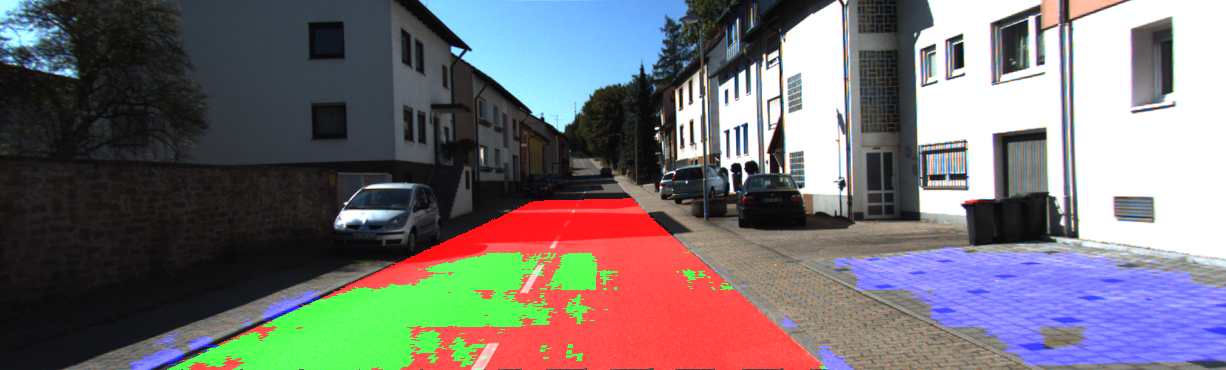
\includegraphics[width=\columnwidth]{figures/kitty_eval/Persp_um_road_000077.png}
        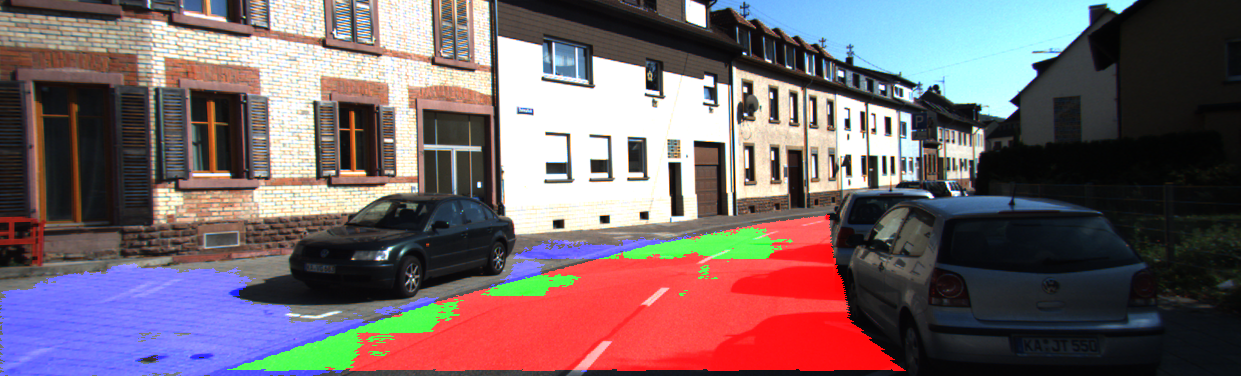
\includegraphics[width=\columnwidth]{figures/kitty_eval/Persp_um_road_000095.png}
        \caption{Shows KITTI test data on which our neural net performed badly. Here, red denotes false negatives, blue areas correspond to false positives and green represents true positives.}
        \label{fig:sfig1}
    \end{subfigure}
    \begin{subfigure}[t]{\columnwidth}
        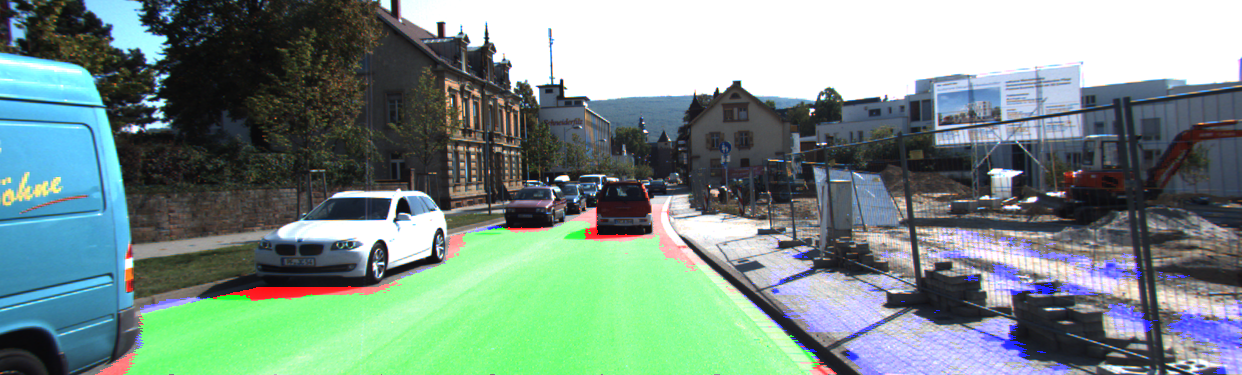
\includegraphics[width=\columnwidth]{figures/kitty_eval/Persp_uu_road_000027.png}
        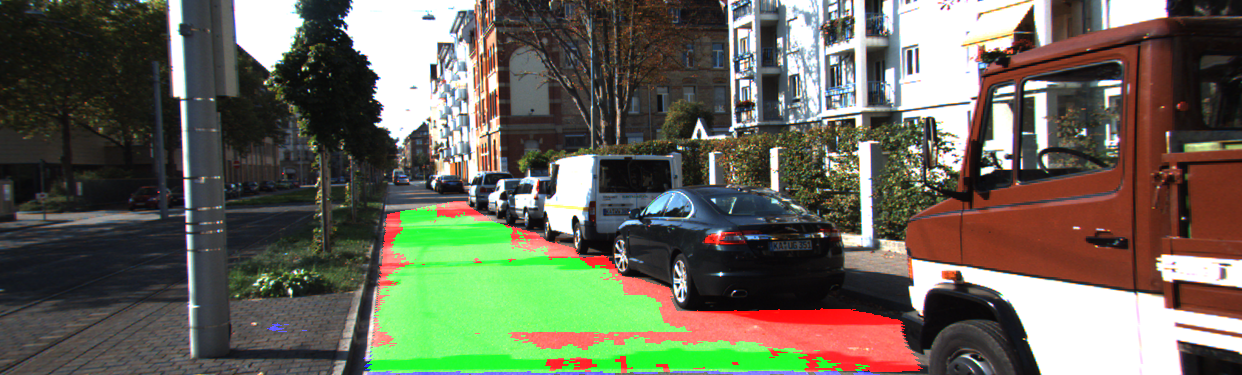
\includegraphics[width=\columnwidth]{figures/kitty_eval/Persp_uu_road_000082.png}
        \caption{Shows KITTI test data on which our neural net performed well.}
        \label{fig:sfig2}
    \end{subfigure}
\end{figure*}




\begin{table*}[]
    \begin{center}
    \begin{tabular}{c|cccccc}
        \toprule
        {\bf Benchmark} & {\bf $\mathbf{F_1}$} & {\bf AP} & {\bf PRE} & {\bf REC} & {\bf FPR} & {\bf FNR}\\
        \midrule
        UM    & \SI{67.91}{\percent} & \SI{61.63}{\percent} & \SI{86.90}{\percent} & \SI{55.74}{\percent} & \SI{3.83}{\percent} \% & \SI{44.26}{\percent}\\
        UMM   & \SI{79.67}{\percent} & \SI{78.41}{\percent} & \SI{93.29}{\percent} & \SI{69.51}{\percent} & \SI{5.50}{\percent} \% & \SI{30.49}{\percent}\\
        UU    & \SI{56.48}{\percent} & \SI{51.89}{\percent} & \SI{84.67}{\percent} & \SI{42.37}{\percent} & \SI{2.50}{\percent} \% & \SI{57.63}{\percent}\\
        URBAN & \SI{71.10}{\percent} & \SI{65.14}{\percent} & \SI{89.83}{\percent} & \SI{58.84}{\percent} & \SI{3.67}{\percent} \% & \SI{41.16}{\percent}\\
        \bottomrule
        \end{tabular}
    \end{center}
    \caption{Results of the official KITTI evaluation. (AP = Average Precision, PRE = Precision, REC = Recall, FPR = False Positive Rate, FNR = False Negative Rate)}
    \label{tab:kitti}
\end{table*}



To evaluate if we could meet our predefined time constraint (classification of
one image in under \SI{20}{\milli\second}) we conducted a run time evaluation
which is shown in \Cref{tab:runtime}. As expected, the runtime increases with a
smaller stride size. The classification model shows an overall faster run time
performance as the regression. Finally, we managed to achieve a run time under
\SI{20}{\milli\second} by using a stride of $s=51$ in both approaches.





As the regression approach had the best performance and also met our time
constraint, we used it to evaluate the KITTI test set and submitted the results
after a transformation into birds eye view (KITTI
specifications).\Cref{tab:kitti} shows the results which are split into the
different road types (UM, UMM, UU, URBAN).
Unfortunately, our regression model performs much worse on the official test
set than on our own test set. Here the $F_1$-measure score ranges between
\SI{56.4}{\percent} and \SI{79.7}{\percent} while Mohan ~\cite{Tarel2009}
achieves on all road categories a $F_1$-measure score of about
\SI{90.0}{\percent}. The reason for this huge difference to might be: \\

\begin{enumerate}
    \item Overfitting of the neural network on our own test data
    \item Specialization of our two models on images with half the original
          size (the KITTI evaluation is done on full size images)
    \item Visible in the two images of \cref{fig:sfig1} is an example of very
          bad performance on a part of the test image data. Basically more
          non-street is classified as street and most of the street is not
          recognized as one at all. This could be due to the fact of shadows
          in some parts of the street and a bit different color of this
          particular street than most of the street our neural network has
          learned in the training.
\end{enumerate}
To improve the latter it would be essential to use training data of a lot more
different street types and lighting conditions.\\
Finally \cref{fig:sfig2} gives some positives example where our neural network
did well. Hardly no false positives and the street around the cars is nicely
segmented.








%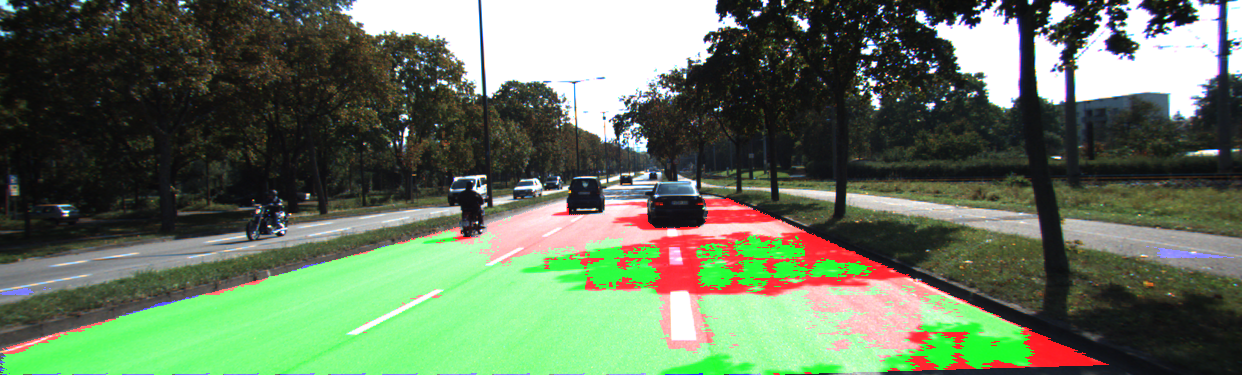
\includegraphics[scale=0.2]{figures/kitty_eval/Persp_umm_road_000025.png}
%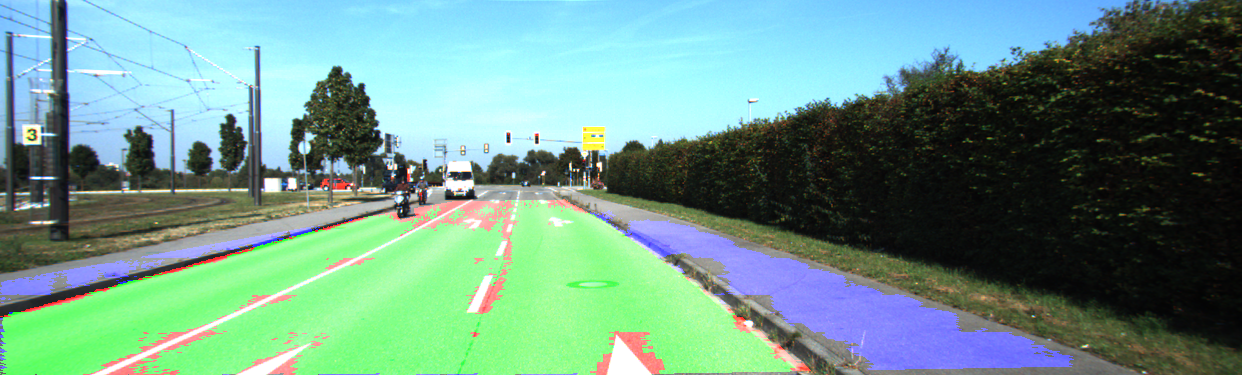
\includegraphics[scale=0.2]{figures/kitty_eval/Persp_umm_road_000040.png}
%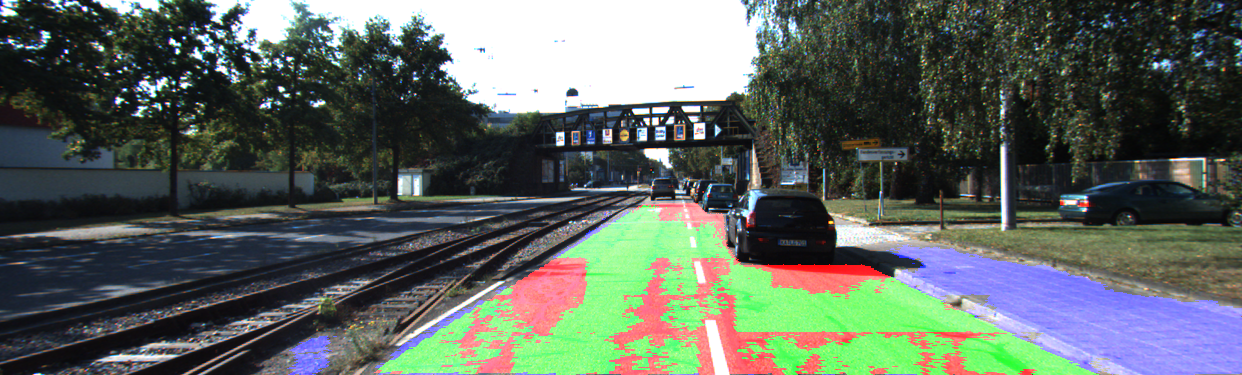
\includegraphics[scale=0.2]{figures/kitty_eval/Persp_umm_road_000066.png}
%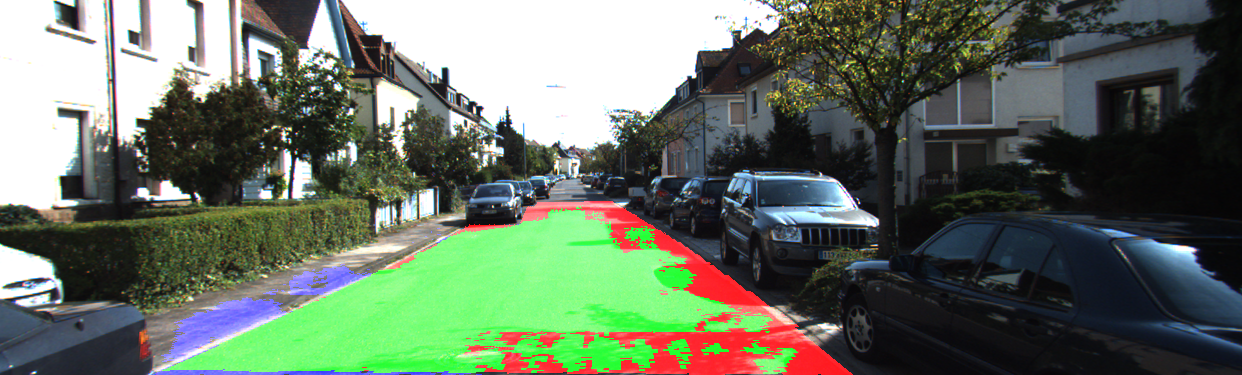
\includegraphics[scale=0.2]{figures/kitty_eval/Persp_uu_road_000020.png}

%!TEX root = pixel-wise-street-segmentation.tex

\section{Conclusion}\label{sec:discussion}

The results presented in this paper were obtained over five months in a
practical course. We started with the Caffe framework and tinkered around with
a fork created by Jonathan Long. The model he provided could not be used on our
computers, because \SI{4}{\giga\byte} of GPU RAM were not enough to evaluate
the model. We tried to adjust the model model, but we failed due to the lack of
documentation, cryptic error messages and random crashes while training or
evaluating. This was the reason why we switched to Lasagne. Using this
framework, we noticed that we still need to try many different topologies. Our
first tries lead to bad classification accuracy and we are not aware of any
analytical way to determine a network topology for a given task. For this
reason, we developed the SST framework. This allows developers to quickly
train, test, and evaluate new network topologies. Although the framework got
its final flexible form in the last month of the practical course, we used it
to evaluate regression and classification models with several topologies. The
results are described in \cref{sec:evaluation}.

In standard scenes, the classification accuracy is impressive. The street gets
segmented very well in a runtime of well below  $\SI{0.5}{\second}$. However,
in some images the model does perform very badly. These are mainly images with
special situations such as an uncommon street colors or unusual lightning. We
believe that these problems can be easily eliminated by using more training
data. Another approach to get better results on the KITTI data set is to train
the model with different data and only use the KITTI training data for
fine-tuning.

One advantage of our models is that they are perfectly parallelizable. Each
image section can be evaluated independently. This can be advantageous in
practical applications. When using specialized hardware such as neuromorphic
chips it is possible to build hundreds of cores in a car. In such a case our
classification approach can yield outstanding results. Given enough training
data (e.g. 1.2~million images) using GoogLeNet or AlexNet can provide perfect
classification results.

Finally one can also improve the results with better hardware. For some of our
models the \gls{GPU} RAM was the limiting factor. Especially for the regression
model using a bigger section of the image can lead to much better results in
quality as well as in speed.



\bibliographystyle{IEEEtranSA}
\bibliography{pixel-wise-street-segmentation}
\end{document}
